\documentclass[10pt,conference]{IEEEtran}

\usepackage{amsmath}
\usepackage{booktabs}
\usepackage{graphicx}
\usepackage{cite}
\usepackage{url}
\usepackage{xcolor}

\begin{document}

\title{Engineered Intelligence for Postoperative Atrial Fibrillation:\\
A ZYAL Agent Fleet, a Stage Grammar, and Genetic Search of\\
Complete Tabular Pipelines on STS Registry Data}

\author{
\IEEEauthorblockN{Jepson Taylor}
\IEEEauthorblockA{NeverHuman Search\\
Scottsdale, AZ, USA\\
jepson@neverhuman.ai}
\and
\IEEEauthorblockN{Zain Khalpey, MD}
\IEEEauthorblockA{HonorHealth\\
Scottsdale, AZ, USA\\
zkhalpey@honorhealth.com}
}

\maketitle

\begin{abstract}
Postoperative atrial fibrillation (POAF) is the most common rhythm
complication of adult cardiac surgery, yet machine-learning prediction from
static surgical-registry variables has plateaued at moderate discrimination.
We ask a sharper question than ``which model is best:'' can an
\emph{engineered-intelligence} (EI) system---one that decomposes the act of
machine learning itself into a formal grammar and then searches that grammar
autonomously---invent \emph{complete} tabular pipelines that \emph{reach} expert
and published baselines while remaining auditable and reproducible, and can it do
so under honest statistical inference? Our EI system
couples (i)~an algorithm decomposition into an eight-stage grammar
(sanitize, scale, expand, select, reduce, sample, model, fuse), (ii)~ZYAL, a
declarative agent-scripting language that governs a supervisor and a fleet of up
to 70 worker agents across 7 users, (iii)~genetic evolution with adversarial
judges, and (iv)~a single-use holdout firewall applied to the confirmation draw.
On a fixed Society of Thoracic
Surgeons (STS) split (10{,}000 train / 3{,}000 holdout; 147 predictors; 9
outcomes), a raw linear-discriminant baseline reaches 0.685 holdout AUROC
(95\% CI 0.664--0.705) and the
strongest non-TabPFN human model reaches 0.681 (95\% CI 0.660--0.700); five
recreated published methods read 0.667--0.683 on \emph{our} cohort. The
license-clean EI champion, E3, attains \textbf{0.689309} holdout AUROC
(95\% CI 0.670--0.709). These confidence intervals overlap heavily: a DeLong test
gives E3 vs.\ baseline $\Delta{=}0.0042$ ($p{=}0.048$, borderline) and E3 vs.\
the best human RF $\Delta{=}0.0087$ ($p{=}0.099$, not significant). The honest
headline is therefore that engineered intelligence \emph{reaches} the
$\sim$0.689 registry-only POAF ceiling but does \emph{not} significantly surpass
strong human baselines; because E3 was itself selected as champion under the same
noisy regime, the winner's curse applies to E3 too. Two \emph{distinct} searches
support this: a 500-generation feature-selection genetic algorithm (this work)
whose CV peaks at 0.7317 (generation~165) while its 3k holdout never escapes
$\sim$0.675--0.690, and a separate MIMO pipeline search of 5{,}917
receipt-audited runs over 200 generations whose generation-169 winner reads 0.697
cross-validation / 0.686 holdout. Across the 500-generation series,
cross-validation does \emph{not} rank holdout performance (Spearman $-0.061$,
$p{=}0.175$)---a decoupling that is the core methodological result and the reason
a held-out firewall matters. A ridge attribution over 5{,}768 deduplicated
genomes explains $R^2{=}0.548$ of selection-score variance and shows that fusion
dominates ($\Delta R^2{=}0.257$), but it predicts the CV objective, not holdout
generalization. E3 is well-calibrated (slope 0.845, intercept $-0.113$, Brier
0.200) with positive decision-curve net benefit. Twenty-four ZYAL-engineered
features survive into E3's mask as cohort-specific signals. On a temporal external
cohort we further find that 24.6\% of holdout rows are feature-identical to
training rows; this leak inflates unregularized trees to AUROC 0.78, but after
de-duplication every method---human and engineered---collapses into a single
0.680--0.689 band, confirming the ceiling out of cohort. The contribution is
not a leaderboard entry; it is a reproducible, auditable characterization of the
POAF ceiling and of the CV--holdout decoupling (and leakage pitfalls) that make
leaderboards misleading.
\end{abstract}

\begin{IEEEkeywords}
engineered intelligence, automated machine learning, agent scripting language,
genetic programming, multi-output learning, holdout firewall, postoperative
atrial fibrillation, Society of Thoracic Surgeons, reproducibility.
\end{IEEEkeywords}

\section{Introduction}
Postoperative atrial fibrillation (POAF) is the most frequent arrhythmic
complication after adult cardiac surgery, with reported incidence commonly in
the range of $20$--$40\%$ depending on procedure, monitoring intensity, and
diagnostic threshold \cite{andrei2024,pandey2023,karri2021}. Its clinical and
economic footprint is large: POAF is independently associated with increased
stroke risk, longer intensive-care and total hospital length of stay, higher
in-hospital and downstream mortality signals, anticoagulation-related
complications, and substantial incremental cost \cite{pandey2023,riad2022,mathew2004}.
Because the rhythm event is downstream of an interacting web of inflammatory,
hemodynamic, autonomic, and structural-remodeling pathways, accurate
preoperative stratification could direct prophylaxis, monitoring, and resource
allocation to the patients most likely to benefit.

Despite decades of effort, the discriminative ceiling for POAF prediction from
\emph{static surgical registry variables} is stubbornly moderate. Classical risk
indices such as the Mathew multicenter index \cite{mathew2004} and the
CHADS/CABG-era scores degrade sharply when transported to new cohorts
\cite{pollock2018}. A systematic review and meta-analysis of published POAF risk
scores reports pooled discrimination that rarely clears the high-$0.6$ band and
is frequently lower on external validation \cite{pandey2023}. Modern
machine-learning studies tell a consistent story: the strongest national STS
analysis of new-onset AF after mitral surgery reports a best test AUROC near the
high-$0.6$s, with regularized logistic regression matching or exceeding random
forest and gradient boosting \cite{andrei2024}; intensive-care and CABG-specific
ML studies report higher numbers only when they add continuous telemetry,
regional cohorts, or richer signal not present in a quality-reporting registry
\cite{karri2021,ma2025,zheng2026,elsherbini2023,kaur2026}. The honest reading is
that registry-only POAF is a \emph{hard} problem and that swapping one
off-the-shelf learner for another moves discrimination very little.

This paper takes a different stance toward that wall. Rather than ask which
\emph{model} is best, we ask whether the act of constructing a machine-learning
pipeline can itself be \emph{decomposed}, \emph{scripted}, and \emph{searched}
by an autonomous system---an \emph{engineered intelligence} (EI). Our EI
decomposes a tabular pipeline into an eight-stage grammar (sanitize, scale,
expand, select, reduce, sample, model, fuse); expresses governance and agent
behavior in ZYAL, a declarative agent-scripting language; dispatches work across
a supervisor and a fleet of up to 70 worker agents shared by 7 users; evolves
candidate genomes with genetic operators and adversarial judges; and protects a
single-use holdout behind a firewall for the final confirmation draw, so that the
reported confirmation number is earned exactly once. (As we make explicit below,
the exploratory evolution series and the benchmark ladder were measured on the 3k
holdout \emph{repeatedly}---as a monitor---which is precisely why they expose
overfitting; the single-use firewall applies only to the COXMAZE final-20
confirmation draw.) The test bed is a fixed STS-derived smoke split
(10{,}000 train / 3{,}000
holdout) with 147 registry predictors and 9 postoperative outcomes; POAF
(\texttt{TARGET\_COtAFib}) is primary and prevails at $33.9\%$ (train) /
$32.8\%$ (holdout); the eight auxiliary labels are used only to train
multi-input/multi-output (MIMO) models and are \emph{never} available at
inference.

Our contributions are: (1)~a formal algorithm decomposition and the ZYAL grammar
that drives it (Section~\ref{sec:ei}); (2)~a supervisor/agent-fleet architecture
with genetic evolution and adversarial judges, and an explicit account of the
\emph{four limits of the human researcher} that motivate it; (3)~ZYAL feature
discovery, including 24 engineered clinical features that survive into the
champion's feature mask (Section~\ref{sec:features}); (4)~the license-clean
champion E3 with a stage-by-stage breakdown and a receipt-corpus stage
attribution (Section~\ref{sec:e3}); and (5)~a reproducibility protocol built
around a single-use holdout firewall for the confirmation draw, with full
statistical inference (95\% CIs, DeLong tests), an unflinching treatment of
cross-validation optimism, the documented \emph{decoupling} of CV from holdout
ranking, and the $\sim$0.689 wall. Throughout, TabPFN~v2.5 is reported
\emph{only} as a human baseline; it appears nowhere in the EI results.

\section{Recreated Published Methods}
\label{sec:recreated}
To anchor the EI against the literature on \emph{identical} data, we recreated
the top families of published POAF and tabular-risk methods and refit them on our
10{,}000/3{,}000 split. We emphasize an honest caveat up front: these are
\emph{recreations of method families on our cohort}, not the original studies.
Because cohort, feature space, missingness policy, and endpoint definition all
differ from the source publications, the recreated numbers read \emph{below}
their published headlines---this is expected and is a property of cohort
transport, not a defect of the original work.

Table~\ref{tab:recreated} reports the five recreations. M3 (a NOPAF/INSPIRE-style
random forest with importance reduction) and M4 (an H2O-AutoML-style stacked
super learner) are the strongest at 0.680609 and 0.682988 holdout AUROC; the
penalized-LASSO POLARIS-style logistic (M2) reaches 0.675825; the
XGBoost-with-Boruta-style reduction (M1, after Shin et al.) reaches 0.671499; and
the COM-AF-style combined risk-score logistic (M5), restricted to 17 score
inputs, reaches 0.666948. The compression of all five into a narrow
0.667--0.683 band mirrors the public literature \cite{andrei2024,pandey2023}: on
registry variables, the choice of learner family is a second-order effect.
Calibration (Brier $0.2006$--$0.2042$) and AUPRC ($0.487$--$0.506$) are likewise
tightly clustered.

\begin{table}[t]
\centering
\caption{Recreated published methods, refit on \emph{our} 10k/3k STS split.
Numbers read below published headlines because the cohort, features, and
endpoint differ.}
\label{tab:recreated}
\footnotesize
\begin{tabular}{@{}lccccc@{}}
\toprule
Method (family) & $n_f$ & CV & Hold. & AUPRC & Brier \\
\midrule
M1 Shin (XGB+Boruta)        & 146 & 0.6699 & 0.6715 & 0.498 & 0.2036 \\
M2 POLARIS (LASSO logit)    & 146 & 0.6822 & 0.6758 & 0.493 & 0.2026 \\
M3 NOPAF/INSPIRE (RF+imp.)  & 146 & 0.6859 & 0.6806 & 0.506 & 0.2008 \\
M4 H2O super learner (stack)& 146 & 0.6910 & 0.6830 & 0.505 & 0.2006 \\
M5 COM-AF (risk-score logit)& 17  & 0.6786 & 0.6669 & 0.487 & 0.2042 \\
\bottomrule
\end{tabular}
\end{table}

\section{Exhaustive Human Models}
\label{sec:human}
We next swept a broad library of \emph{single-stage} human models---no pipeline
search, no engineered features, the same 147-predictor matrix, the same seed and
row order, and folds-internal preprocessing---to establish the strongest result a
competent human achieves by ``picking a good classifier.'' Of 33 models,
Table~\ref{tab:human} lists the top eight by holdout AUROC. The best is a tuned
TabPFN classifier at 0.683203, followed by a random forest at 0.682778 and an
AutoGluon ensemble at 0.681039. A GPU TabPFN~v2.5 run (n32) reaches 0.679688;
linear discriminant analysis and logistic regression sit at 0.674061 and
0.672968. The strongest human model (0.683) is statistically indistinguishable
from the raw LDA-112 baseline of 0.685153, and the entire competitive human band
is compressed into roughly one AUROC point---well inside the Hanley--McNeil
single-AUROC standard error of $\sim$0.0107 at this sample size and prevalence
($n{=}3000$, prev.\ 0.328; Section~\ref{sec:results}). A refit random-forest
baseline (0.680609, the comparator used for the E3-vs-human DeLong test) carries a
95\% CI of $[0.660, 0.700]$ that overlaps both the LDA-112 baseline and E3 (the
strongest catalog human classifier, RandomForestBinaryClassifier at 0.682778, sits
in the same band). We stress again: \textbf{TabPFN~v2.5 is a human baseline
only}; it is excluded from every engineered-intelligence claim, figure, and
headline that follows.

\begin{table}[t]
\centering
\caption{Top human single-stage models (no pipeline search). TabPFN v2.5 (GPU)
is a \emph{baseline only} and is excluded from all EI results.}
\label{tab:human}
\footnotesize
\begin{tabular}{@{}lc@{}}
\toprule
Human model (no pipeline) & Holdout AUROC \\
\midrule
TabPFNClassifier                    & 0.683203 \\
RandomForestBinaryClassifier        & 0.682778 \\
AutoGluonClassifier                 & 0.681039 \\
TabPFN\_v2.5\_n32\_GPU (baseline)   & 0.679688 \\
RandomForestBaseline                & 0.678816 \\
LinearDiscriminantBinaryClassifier  & 0.674061 \\
TabPFN\_v2.5\_n16\_GPU (baseline)   & 0.673091 \\
LogisticRegressionBaseline          & 0.672968 \\
\bottomrule
\end{tabular}
\end{table}

\section{AutoML and the Reality of the Holdout}
\label{sec:automl}
The natural next step is automated machine learning: let a search optimize over
learners and hyperparameters. AutoML can recover incremental signal, but it
exposes a methodological trap that is central to this paper. When a search
maximizes a cross-validation (CV) score over hundreds of candidates, the maximum
is biased \emph{upward}: it captures both true signal and the lucky tail of
estimation noise. This is the optimism-of-the-maximum, or ``winner's curse,'' a
direct consequence of selecting on a noisy objective \cite{bergstra2012,hutter2019}.

Figure~\ref{fig:evolution} makes the hazard concrete. Over 500 generations of our
\texttt{lda500} feature-selection genetic algorithm (this work, the COXMAZE GA
over LDA-feature masks), the selection (CV) AUROC climbs into the $0.71$--$0.73$
range and peaks at \textbf{0.7317 at generation~165}, while the \emph{held-out}
AUROC for the same genomes never escapes the $\sim$0.675--0.690 band. Crucially,
this per-generation holdout was a \emph{repeatedly measured monitor}, not a
single-use number---which is exactly why it is able to expose overfitting. The gap
between the blue selection curve and the red holdout curve is not
progress---it is optimism. Any pipeline chosen because it topped CV inherits that
inflation. This is why our protocol (Section~\ref{sec:e3}) treats CV as a
\emph{candidate-generation} signal only, gated by paired train-only comparisons,
and reserves a separate single-use firewall for the confirmation draw
(Section~\ref{sec:results}). We emphasize that this \texttt{lda500} GA is a
\emph{different} search from the Codex MIMO pipeline search discussed in
Section~\ref{sec:e3} (whose generation-169 winner reads 0.697 CV / 0.686
holdout); the two should not be conflated.

\begin{figure}[t]
\centering
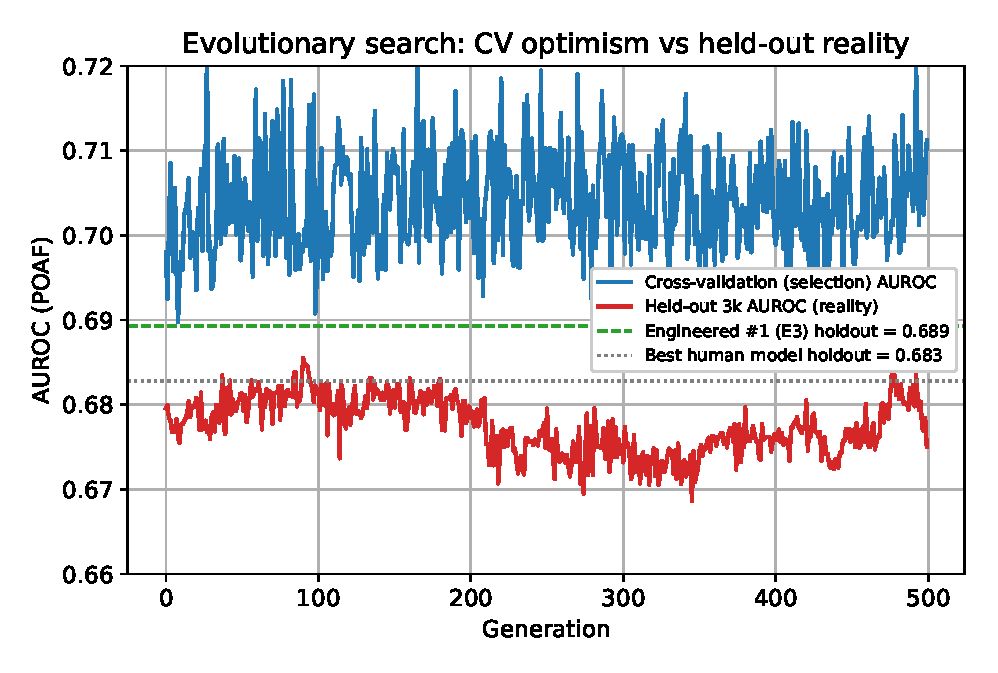
\includegraphics[width=\columnwidth]{figures/fig1_evolution}
\caption{Cross-validation optimism vs.\ held-out reality across the 500-generation
\texttt{lda500} feature-selection GA (this work). Selection AUROC peaks at
$0.7317$ (generation~165) while holdout AUROC stays in the $\sim$0.675--0.690
band. The per-generation holdout here is a \emph{repeatedly measured monitor}
(not the single-use firewall), which is why the widening blue-vs-red gap directly
exposes the winner's curse. This GA is distinct from the Codex MIMO pipeline
search of Section~\ref{sec:e3} (gen-169 winner 0.697 CV / 0.686 holdout).}
\label{fig:evolution}
\end{figure}

Figure~\ref{fig:cvholdout} plots the same phenomenon as a per-generation scatter,
and the statistics are stark enough to constitute a standalone result.
\textbf{Cross-validation is not a valid ranking signal here.} Over the
500-generation series, the rank correlation between CV and holdout is
$\text{Spearman}{=}-0.061$ ($p{=}0.175$) and $\text{Pearson}{=}-0.039$---both
indistinguishable from zero, and if anything weakly \emph{negative}. The point is
sharpened by a partition: the mean holdout AUROC of the top-50 genomes \emph{by
CV} is 0.6775, of the bottom-50 by CV is also 0.6775, and of all genomes is again
0.6775. In other words, knowing a genome's CV rank tells you nothing about its
holdout performance. This is precisely why a held-out firewall matters and why CV
leaderboards mislead: selecting the CV maximum selects for estimation noise as
much as for signal. The practical lesson governs the rest of the paper: a credible
EI must confirm on a held-out number that the CV objective never touched.

\begin{figure}[t]
\centering
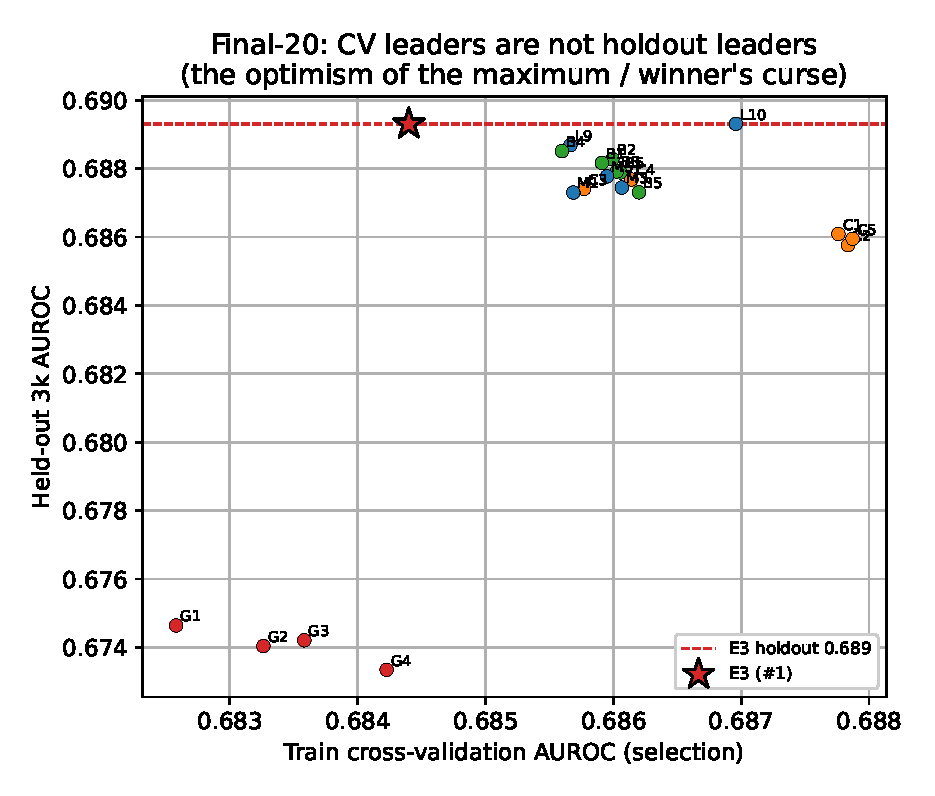
\includegraphics[width=\columnwidth]{figures/fig3_cv_vs_holdout}
\caption{CV (selection) AUROC vs.\ holdout AUROC per genome over the
500-generation series. The two axes are decoupled: Spearman $-0.061$ ($p{=}0.175$),
Pearson $-0.039$; top-50-CV mean holdout (0.6775) equals bottom-50-CV (0.6775)
equals overall (0.6775). Ranking on CV alone selects for noise as much as for
signal \cite{bergstra2012}, which is why CV cannot serve as a ranking signal and a
held-out firewall is required.}
\label{fig:cvholdout}
\end{figure}

\section{Engineered Intelligence}
\label{sec:ei}
We define \emph{engineered intelligence} as the autonomous, receipt-audited
\emph{invention} of complete algorithms in response to a dataset. Where AutoML
tunes a model, EI decomposes the construction of a model into a grammar and
searches that grammar with a fleet of agents under explicit governance. Three
ingredients make this concrete: an algorithm decomposition, an agent scripting
language (ZYAL), and a supervisor/agent-fleet architecture with genetic
evolution. Figure~\ref{fig:zyal} shows the end-to-end workflow.

\subsection{Algorithm decomposition: the stage grammar}
A candidate pipeline is a typed sequence over eight macro stages, each drawn from
a registry of interchangeable operators:
\begin{quote}\footnotesize
\texttt{sanitize $\rightarrow$ scale $\rightarrow$ expand $\rightarrow$ select
$\rightarrow$ reduce $\rightarrow$ sample $\rightarrow$ model $\rightarrow$
fuse}.
\end{quote}
Operationally the genome carries a richer slotting---surrogate, sanitizer,
scaler, two expansion slots, feature selector, reducer, sampler, a primary and
optional secondary model, and a fusion head---so that a candidate may be as
conservative as ``null-sanitize $\rightarrow$ standard-scale $\rightarrow$
logistic'' or as structured as ``high-missingness drop $\rightarrow$
visibility-graph expand $\rightarrow$ gradient-boosting-importance reduce
$\rightarrow$ MIMO primary $+$ decision-tree secondary $\rightarrow$ logistic
stacking.'' Each stage is a \emph{compositional unit}: the search reasons about
combinations of operators, not just a single estimator's knobs. This is the key
departure from AutoML and the reason stage-level attribution
(Section~\ref{sec:e3}) is even possible.

\subsection{ZYAL: an agent scripting language and grammar}
ZYAL is a declarative scripting language that serves as the \emph{governing
context} for the fleet---a runbook, not an imperative program. A ZYAL document
binds three things: (i)~the \emph{search space}, by declaring which operators are
admissible in each stage slot and any license or compute constraints on them;
(ii)~the \emph{evaluation contract}, by declaring the primary endpoint, the
auxiliary-label policy (auxiliary outcomes may be training labels but never
inference inputs), the CV protocol, and the holdout firewall rule; and (iii)~the
\emph{agent behavior}, by declaring how candidates are proposed, judged,
mutated, and promoted. The grammar is small and typed, which makes runs
reproducible: a ZYAL runbook plus a seed deterministically reconstructs the
admissible space and the gating rules. A Python supervisor compiles the runbook
and acts as the \emph{judge of record}, so that no agent can unilaterally
declare a winner.

\subsection{Supervisor and agent fleet}
The supervisor dispatches work to a fleet of up to 70 worker agents shared across
7 users. Workers materialize candidate genomes---each a complete pipeline plus
any engineered features it requests---fit them under the train-only CV contract,
and return receipts. A receipt records the generation, candidate kind
(MISO/MIMO), every stage operator, the selected models, the CV/selection score,
the holdout score when (and only when) the firewall permits, and a genome
fingerprint for deduplication. The receipt corpus is the audit trail that turns a
leaderboard into a \emph{dataset of experiments}.

\subsection{Genetic evolution and adversarial judges}
Candidate genomes evolve under standard genetic operators---mutation of stage
operators, recombination of stage sub-sequences, and fitness-proportional
selection---in the lineage of genetic algorithms and genetic programming
\cite{holland1975,koza1992}, neuroevolution \cite{stanley2002}, and from-scratch
algorithm evolution \cite{real2020}. Before a candidate consumes compute, a panel
of \emph{adversarial judges} can \emph{block} ill-typed or leakage-prone genomes,
\emph{pool} near-duplicates, or \emph{improve} a candidate by proposing a small
edit. The supervisor then applies train-only CV gates---including paired
$\Delta$-versus-champion comparisons and DeLong tests on AUROC---so that
promotion requires evidence beyond a single CV point estimate. Only after all
training-side gates pass does the holdout firewall release a single, report-only
verification.

\begin{figure*}[t]
\centering
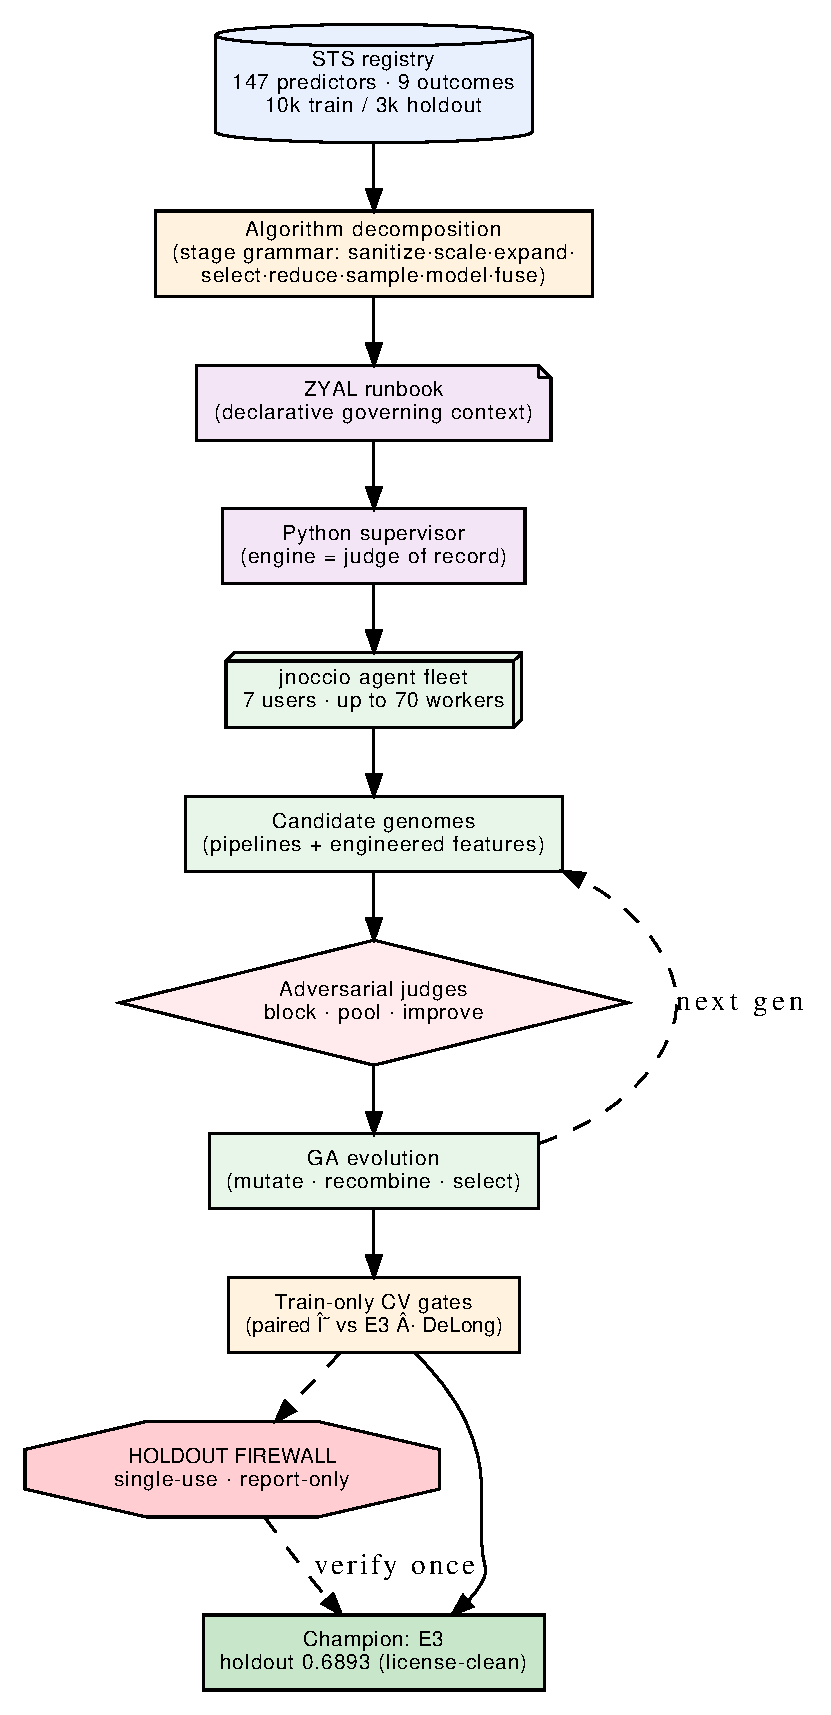
\includegraphics[width=0.66\textwidth]{figures/fig5_zyal_workflow}
\caption{The engineered-intelligence workflow. The STS registry feeds an
algorithm decomposition (stage grammar); a ZYAL runbook supplies the declarative
governing context; a Python supervisor (the judge of record) drives a jnoccio
agent fleet (7 users, up to 70 workers) that materializes candidate genomes;
adversarial judges block/pool/improve; genetic evolution mutates, recombines, and
selects; train-only CV gates use paired $\Delta$-vs-E3 and DeLong tests; and a
single-use holdout firewall is reserved for the COXMAZE final-20 confirmation draw
(lock $+$ DeLong) that confirms the license-clean champion E3 (holdout 0.6893).
The exploratory evolution series and benchmark ladder, by contrast, were measured
on the 3k holdout repeatedly as a monitor.}
\label{fig:zyal}
\end{figure*}

\subsection{The four limits of the human researcher}
The case for EI is not aesthetic; it is a response to four concrete bottlenecks
that bound human-driven discovery.

\emph{(a) Knowledge consumption.} The biomedical literature now grows faster than
any individual can read; bibliometric estimates put modern scientific output
growth at several percent per year, doubling on a timescale of roughly a decade
\cite{bornmann2015}. No surgeon-scientist can hold the full space of candidate
features, operators, and prior results in working memory. An agent fleet can
ingest and operationalize that corpus as admissible operators and engineered
features.

\emph{(b) Hypothesis generation.} A human proposes a handful of hypotheses per
project; the EI proposes thousands of \emph{complete pipelines}, each a structured
hypothesis about how to represent and combine registry signal. The combinatorial
stage grammar makes the hypothesis space explicit and traversable.

\emph{(c) Idea validation time and quality.} A human validates one idea at a time,
slowly, and is tempted to stop at the first ``good enough'' result. The fleet
validates in parallel under a uniform, leakage-safe contract, so that thousands of
ideas are scored on identical terms and the comparison is fair by construction.

\emph{(d) Cognitive bias.} Human analysis is vulnerable to the garden of forking
paths, selective reporting, and confirmation bias---mechanisms shown to make a
large fraction of published findings fragile or false
\cite{ioannidis2005,gelman2014}. The EI does not remove statistical optimism (the
winner's curse is real, Section~\ref{sec:automl}), but it makes the selection
procedure \emph{explicit and replayable}: the firewall, the paired gates, and the
receipt corpus convert ad-hoc judgment into an auditable protocol.

\section{ZYAL Feature Discovery}
\label{sec:features}
Beyond pipeline search, ZYAL agents propose \emph{engineered clinical features}.
Research nodes mine the literature into candidate formulas with citations; each
candidate passes an admission screen that is permutation-null aware, demands
marginal lift, and is strictly leakage-safe and train-only
(Figure~\ref{fig:feature}). A genetic/LDA selection then compresses the augmented
substrate ($196$ features $=$ $146$ raw $+$ $50$ ZYAL-engineered) down to a
$112$-feature mask. Of the 50 proposals, \textbf{24 engineered features survive}
into the champion's mask, indicating that they carry non-redundant
\emph{cohort-specific} signal in this cache. We are careful not to over-read this:
all feature--target correlations reported below are \emph{train-only marginal
associations}, the surviving features are best understood as cohort-specific
signals rather than established physiology, and (as we argue below) the dominant
``young-age'' theme reflects a cohort \emph{selection} structure that we do not
expect to generalize. The clinical rationales we give are \emph{hypotheses}
motivated by each feature's formula and its train-only correlation, not claims
established by citation.

\begin{figure*}[t]
\centering
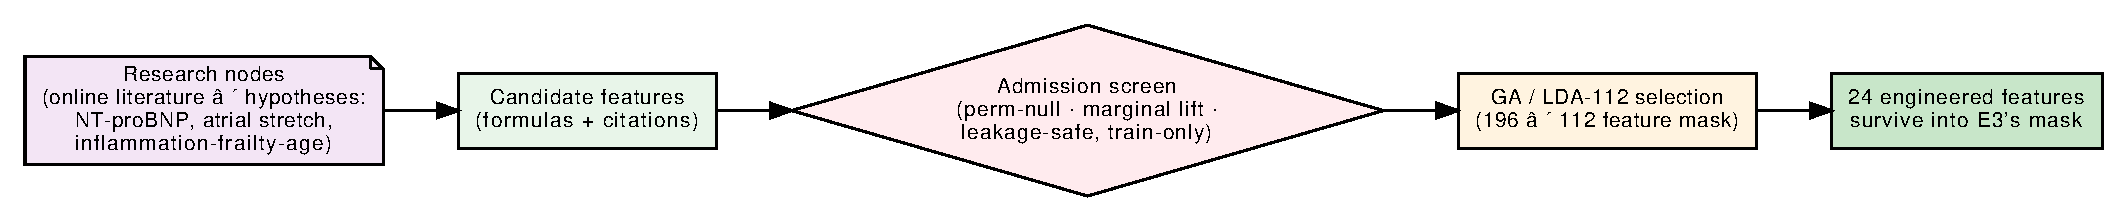
\includegraphics[width=0.92\textwidth]{figures/fig6_feature_discovery}
\caption{ZYAL feature discovery. Research nodes turn literature into candidate
formulas with hypothesized rationales (NT-proBNP missingness, atrial stretch,
inflammation--frailty--age); an admission screen enforces permutation-null,
marginal-lift, leakage-safe, train-only criteria; GA/LDA selection reduces
$196\rightarrow112$; 24 engineered features survive into E3's mask as
cohort-specific signals (train-only marginal associations).}
\label{fig:feature}
\end{figure*}

Several illustrative survivors are listed below with their formula and their
\emph{train-only} marginal correlation with POAF. The accompanying interpretations
are hypotheses motivated by the formula, not established mechanisms:

\begin{itemize}
\item \textbf{\texttt{metabolicriskcalcul}} (train-only corr $-0.253$):
$\text{Age}\cdot\text{BSA}+\text{INR}$. The strongest single engineered
correlate, and notably \emph{negative}---a re-encoding of the cohort's young-age
selection structure (see below).
\item \textbf{\texttt{age\_young\_sick\_score}} (train-only corr $-0.2081$):
\texttt{Age $-$ $10\cdot$(Diabetes$+$PrevMI$+$CHF$+$Depression)}. Flags younger
patients carrying a heavy comorbidity burden; in this cache that subgroup is
associated with higher POAF, but this tracks who was referred to surgery here
rather than a general physiological law.
\item \textbf{\texttt{young\_age\_hscrp\_inflammation\_ratio}} (train-only corr
$-0.1491$): $\text{hsCRP}/(70-\text{Age})$. Hypothesis: inflammation co-varies
with the young, sicker surgical subgroup in this cohort.
\item \textbf{\texttt{cardiac\_workup\_intensity\_frailty\_discordance}}
(train-only corr $0.1536$): a count of non-missing workup fields (HDEF, LVEDD,
PASYS, BNP, NYHA) scaled by youth and inverse-CRP. A
\emph{selective-missingness} signal: which tests were ordered is itself
informative in this cache. This is a center-/workflow-specific encoding, not a
portable biomarker.
\item \textbf{\texttt{lv\_edd\_ef\_ratio\_age\_factor}} (train-only corr
$0.1463$): $(\text{LVEDD}/\text{HDEF})\cdot(70-\text{Age})$. Hypothesis: an
atrial-stretch proxy weighted toward younger patients.
\item \textbf{\texttt{young\_age\_valve\_burden\_interaction}} (train-only corr
$0.1399$): $\max(0,60-\text{Age})\cdot(\text{VDInsufM}+\text{VDInsufT})$. An
age$\times$valve-regurgitation interaction---consistent with younger patients in
this cache being enriched for valve cases.
\item \textbf{\texttt{renal\_function\_albumin\_oxygen\_delivery\_index}}
(train-only corr $-0.1385$): albumin$\cdot$Hct over creatinine, penalized by high
CRP and low EF. An anemia/oxygen-delivery and hypoalbuminemia axis.
\item \textbf{\texttt{inflammatory\_oxygen\_delivery\_gap}} (train-only corr
$0.1233$):
$(\text{hsCRP}/\text{albumin})\cdot(\text{Hb deficit}/\text{Hct})$,
fusing inflammation with anemia.
\item \textbf{\texttt{beta\_blocker\_withdrawal\_age\_factor}} (train-only corr
$0.1627$): peri-operative $\beta$-blocker cessation; hypothesized adrenergic
surge, again weighted toward younger patients.
\end{itemize}

\paragraph{The young-age inversion is a cohort selection confound, not discovered
physiology} A consistent theme across these survivors is that, \emph{in this
surgical research cache}, Age is \emph{negatively} associated with POAF and the
most predictive engineered constructs flag younger patients with disproportionate
comorbidity, inflammation, anemia, or valvular burden. This inverts population
epidemiology, where \emph{older} age increases POAF risk. The most parsimonious
explanation is referral/collider selection: younger patients reaching this
surgical cohort are enriched for sicker and more emergent (often valve) cases, so
conditioning on ``being in this cohort'' induces a spurious young--sick--POAF
association. The engineered ``young-age'' features therefore \emph{re-encode a
cohort-specific selection structure}; we do not interpret them as rediscovered
biology and we do not expect them to transport. They are reported here as
cohort-specific signals---useful within this cache, a cautionary example out of
it.

\section{The \#1 Model: E3}
\label{sec:e3}
The deployable, license-clean champion is \textbf{E3}. Its stage realization is
(Figure~\ref{fig:e3}):
\begin{quote}\footnotesize
\texttt{LDA-112 mask $\rightarrow$ BrownianBridgeRankExpander $\rightarrow$
MonotoneRunAtlasExpander $\rightarrow$ TopologicalSubspaceClassifier}.
\end{quote}

\emph{Substrate and selection.} The $196$-feature substrate ($146$ raw $+$ $50$
ZYAL-engineered) is reduced to the LDA-112 mask; $24$ engineered features survive
(Section~\ref{sec:features}).

\emph{BrownianBridgeRankExpander (BBR).} Adds $+10$ rank/bridge descriptors that
encode each feature's order statistics and bridge-interpolated rank deviations,
giving downstream stages monotone, distribution-robust coordinates.

\emph{MonotoneRunAtlasExpander (MRA).} Adds $+12$ monotone-run descriptors that
catalog the lengths and directions of monotone runs across the ranked
representation, exposing local shape structure that a linear head would miss.

\emph{TopologicalSubspaceClassifier.} A license-clean MIMO head that learns a
shared subspace across all 9 outcomes; the 8 auxiliary outcomes act purely as
training labels and are \emph{never} supplied at inference. The shared
representation regularizes the POAF boundary using correlated complication
structure without ever leaking future facts.

E3 reaches \textbf{holdout AUROC 0.689309} (95\% CI $[0.670, 0.709]$; CV
$\sim$0.6846). Numerically it sits at the top of the benchmark ladder
(Section~\ref{sec:results}), but the appropriate reading is that it \emph{reaches
the same ceiling} as the raw LDA-112 baseline (0.685153, CI $[0.664, 0.705]$) and
the strongest human and recreated methods rather than meaningfully exceeding them.
A DeLong test gives E3 vs.\ baseline $\Delta{=}0.0042$ (95\% CI $[4{\times}10^{-5},
0.0083]$, $p{=}0.048$, borderline) and E3 vs.\ the best human RF $\Delta{=}0.0087$
(95\% CI $[-0.0016, 0.0190]$, $p{=}0.099$, not significant). We do \emph{not}
exempt E3 from the winner's curse: E3 was selected as champion under the same
noisy CV regime that inflates any maximum, so its small numerical edge is not
robustly significant and should be read as ``indistinguishable from the registry
ceiling,'' not as a superior predictor.

\begin{figure*}[t]
\centering
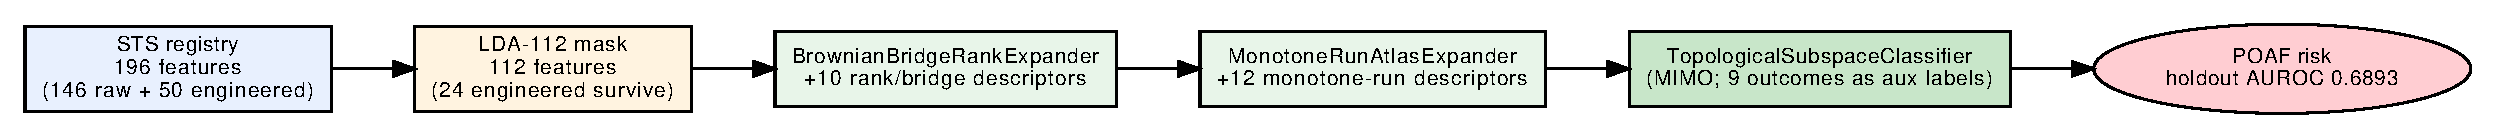
\includegraphics[width=0.96\textwidth]{figures/fig7_e3_pipeline}
\caption{The champion E3 (license-clean), stage by stage. A $196$-feature
substrate ($146$ raw $+$ $50$ engineered) is masked to LDA-112 ($24$ engineered
features survive), expanded by BrownianBridgeRankExpander ($+10$ rank/bridge
descriptors) and MonotoneRunAtlasExpander ($+12$ monotone-run descriptors), and
classified by a TopologicalSubspaceClassifier (MIMO; 9 outcomes as auxiliary
labels, none used at inference) for a holdout AUROC of 0.6893.}
\label{fig:e3}
\end{figure*}

\subsection{Stage attribution from the receipt corpus}
A separate Codex EI MIMO search---\emph{distinct} from the \texttt{lda500}
feature-selection GA of Section~\ref{sec:automl}---produced a large receipt
corpus: $5{,}917$ receipt-audited runs over $200$ generations, $5{,}768$
deduplicated genomes. Its generation-169 winner
(AxiomForgeCopulaWeaverClassifier: high-missingness
drop $+$ visibility-graph expand $+$ gradient-boosting-importance reduce $+$
decision-tree secondary $+$ logistic stacking fusion) reached $0.697$ CV /
$0.686$ holdout. The corpus lets us treat ``what made a pipeline
win?'' as its \emph{own} regression problem. We fit a ridge model that predicts a
genome's \emph{selection (CV) AUROC} from its stage choices; it explains
$R^2{=}0.548$ of that variance.

\textbf{What this attribution does and does not say.} The ridge predicts the
\emph{selection objective}, i.e.\ CV/selection AUROC---which, as
Section~\ref{sec:automl} showed, is essentially \emph{uncorrelated} with holdout
in this regime (Spearman $-0.061$). The attribution therefore explains
\emph{what won the noisy CV objective}, not what generalizes to the holdout. It is
moreover \emph{observational} over search-selected genomes: because genomes are
retained on the basis of their score, conditioning on the surviving population is
collider-prone, so the coefficients are associational, not causal. We report it as
an interpretable map of the search's preferences, not as evidence that fusion
``causes'' generalization.

The macro-stage attribution (the drop in $R^2$ when a stage is ablated from the
ridge) is unambiguous: \textbf{fusion dominates} with $\Delta R^2{=}0.2566$,
followed distantly by the reducer ($0.0200$) and the primary model ($0.0080$);
all remaining stages contribute under $0.003$ each (Table~\ref{tab:attr},
Figure~\ref{fig:attr}). Among individual operators, the largest positive
coefficients are LogisticStackingFusion and RidgeStackingFusion, the MIMO model
family, and supervised reducers (RandomForestProximityReducer,
GradientBoostingImportanceReducer). The discovered \emph{pattern}---learn a
useful representation, reduce with supervised importance, then \emph{fuse}
complementary predictors with a stacking head \cite{wolpert1992}---is a plausible
recipe for scoring well on a noisy CV objective, where ensembling stabilizes
estimation. It is an interpretability result of a different kind: not which feature
mattered to a model, but which \emph{stage of model construction} the search
rewarded---bearing in mind that the rewarded objective (CV) does not predict
holdout here.

\begin{table}[t]
\centering
\caption{Macro-stage attribution: drop in cross-validated ridge $R^2$
($R^2_{\text{full}}{=}0.548$) when each stage is ablated. Fusion dominates.}
\label{tab:attr}
\footnotesize
\begin{tabular}{@{}lc@{}}
\toprule
Macro stage & $\Delta R^2$ \\
\midrule
Fusion              & 0.2566 \\
Reducer             & 0.0200 \\
Primary model       & 0.0080 \\
Secondary model     & 0.0026 \\
Feature selector    & 0.0020 \\
Scaler              & 0.0015 \\
Sanitizer           & 0.0009 \\
Expansion II        & 0.0001 \\
\bottomrule
\end{tabular}
\end{table}

\begin{figure}[t]
\centering
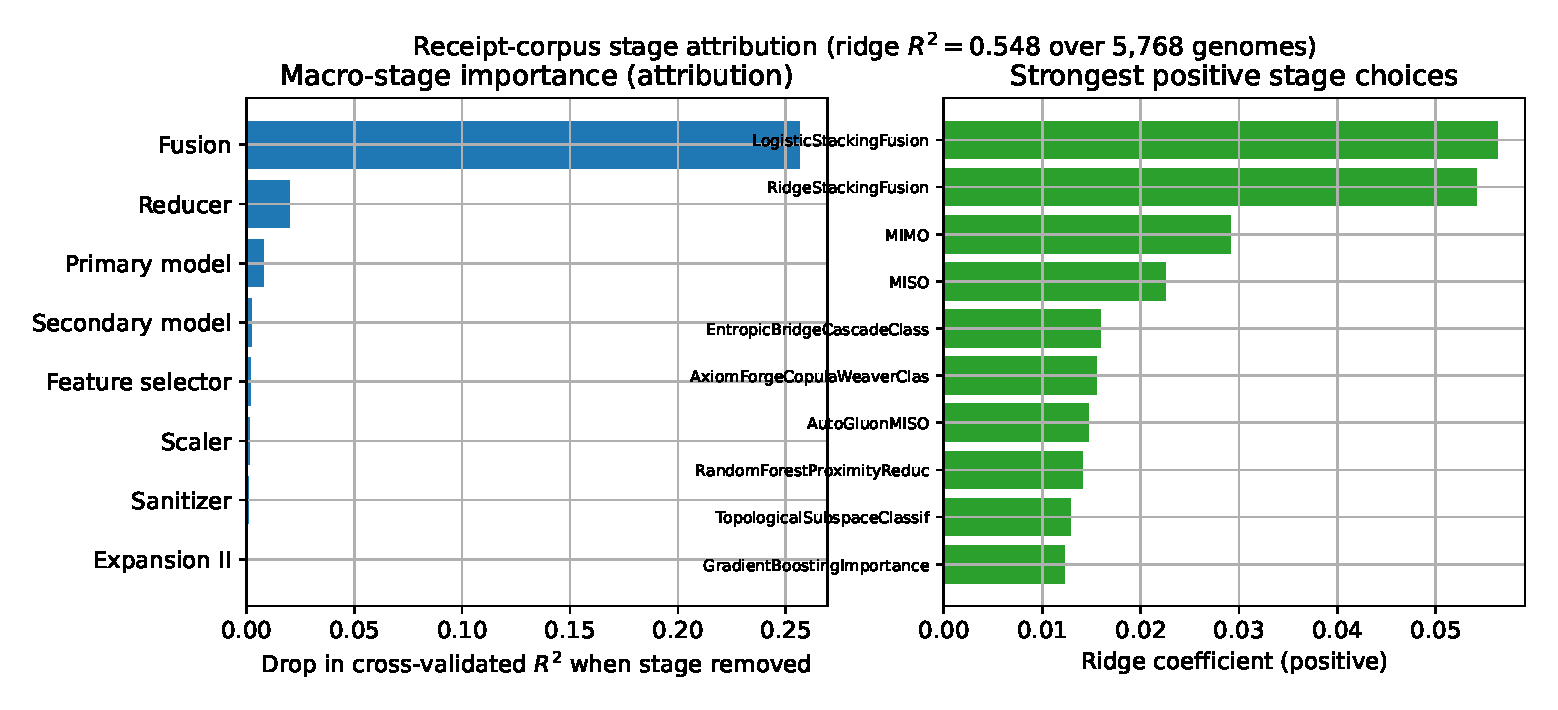
\includegraphics[width=\columnwidth]{figures/fig4_stage_attribution}
\caption{Stage attribution over the receipt corpus ($5{,}768$ deduplicated
genomes). Left: macro-stage $\Delta R^2$ for a ridge predicting selection AUROC
($R^2{=}0.548$); fusion dominates. Right: the largest positive per-operator
coefficients (stacking fusions, MIMO family, supervised reducers).}
\label{fig:attr}
\end{figure}

\section{Results}
\label{sec:results}
Table~\ref{tab:ladder} and Figure~\ref{fig:ladder} present the benchmark ladder
on the fixed 3{,}000-row holdout. E3 sits numerically at the top (0.689309),
ahead of the
AxiomForge MIMO winner (0.6858), the raw LDA-112 baseline (0.685153), the best
human model (0.683203), and all recreated published methods (top recreation
0.682988). The generation-0 MISO baseline (0.667) and the COM-AF-style logistic
(0.666948) anchor the bottom. But the entire competitive field spans roughly two
AUROC points---comfortably inside the Hanley--McNeil single-AUROC standard error
of $\sim$0.0107 at this $n{=}3000$, prevalence-0.328 holdout---so the ladder is
better read as a cluster at a shared ceiling than as a ranking. The inference of
Section~\ref{sec:e3} applies: E3 vs.\ baseline is borderline ($p{=}0.048$) and
E3 vs.\ the best human RF is not significant ($p{=}0.099$).

\paragraph{Multiplicity context for the winner's curse} This ladder, and the
champion atop it, were obtained by scoring \emph{thousands} of distinct models
against the same 3k holdout: 33 human single-stage models, 5 recreated published
methods, the COXMAZE final-20 confirmation set, the 500 generations of the
\texttt{lda500} GA, and the Codex 5{,}917-run corpus. With that many comparisons
against one holdout, an apparent maximum is expected to drift above the truth---the
multiple-comparisons setting in which the winner's curse operates and in which a
$\sim$0.0042 edge ($p{=}0.048$) cannot be treated as a robust win. Accordingly,
the single-use holdout firewall (lock $+$ DeLong) was reserved for the COXMAZE
final-20 confirmation draw only; the per-generation evolution holdout and the
benchmark ladder were measured on the 3k repeatedly, as a monitor.

\begin{table}[t]
\centering
\caption{Benchmark ladder on the fixed 3k holdout. EI champion E3 is numerically
highest, but the whole field lies within $\sim$1 Hanley--McNeil SE ($\sim$0.0107);
differences are not robustly significant (see Section~\ref{sec:e3}). TabPFN
appears only as a human baseline.}
\label{tab:ladder}
\footnotesize
\begin{tabular}{@{}llc@{}}
\toprule
Entry & Category & Holdout AUROC \\
\midrule
EI \#1: E3 (license-clean)        & engineered & \textbf{0.689309} \\
EI: AxiomForge MIMO (Codex)       & engineered & 0.6858 \\
Raw LDA-112 baseline              & baseline   & 0.685153 \\
Human: TabPFNClassifier           & human      & 0.683203 \\
Recreated: H2O super learner      & recreated  & 0.682988 \\
Human: RandomForestBinary         & human      & 0.682778 \\
Human: AutoGluonClassifier        & human      & 0.681039 \\
Recreated: NOPAF/INSPIRE (RF)     & recreated  & 0.680609 \\
Human: TabPFN v2.5 (GPU)          & human      & 0.679688 \\
Recreated: POLARIS (LASSO logit)  & recreated  & 0.675825 \\
Recreated: Shin (XGB+Boruta)      & recreated  & 0.671499 \\
EI: gen-0 MISO best               & engineered & 0.667 \\
Recreated: COM-AF (risk-score)    & recreated  & 0.666948 \\
\bottomrule
\end{tabular}
\end{table}

\begin{figure}[t]
\centering
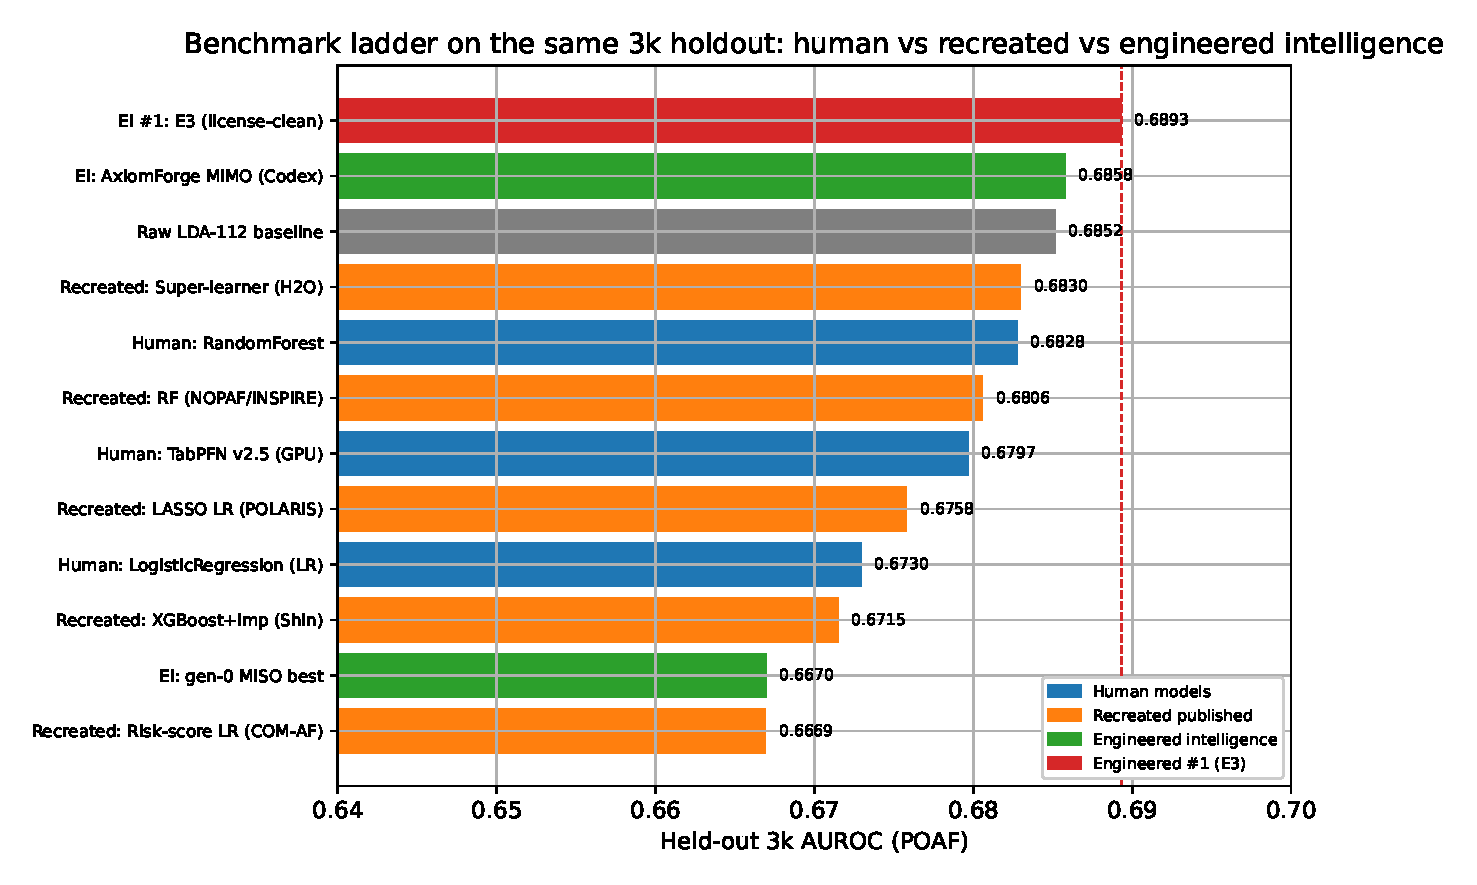
\includegraphics[width=\columnwidth]{figures/fig2_benchmark}
\caption{Benchmark ladder on the fixed 3k holdout. The license-clean EI champion
E3 (0.689309) is numerically highest, but the whole field spans $\sim$2 AUROC
points---within one Hanley--McNeil SE ($\sim$0.0107)---so it reaches, rather than
clears, the registry-only POAF ceiling.}
\label{fig:ladder}
\end{figure}

\section{Does the Top Model Transfer to a Larger Dataset? The 50k/10k Test}
\label{sec:transfer}
A pipeline selected on a $10{,}000/3{,}000$ split invites a scaling question: does
the discovery champion remain the champion when retrained on $5\times$ the data and
tested on a larger, later cohort? We test it directly. We rebuild the EI pipeline
end-to-end---ZYAL feature engineering and the LDA-112 downsample \emph{re-derived} on
the new data---and retrain the champion E3, the top-CV pipelines (C1, C2), and three
recreated methods on a $\mathbf{49{,}999}$-operation training set, evaluating on a
$\mathbf{2017}$ holdout of $\mathbf{10{,}000}$ operations. Human/recreated comparators
again receive only raw default features. This is simultaneously a scale test ($5\times$
training data) and a temporal external test.

\paragraph{Leakage audit first.} The larger split contains a data-quality flaw we
report transparently: \textbf{$2{,}463/10{,}000$ ($24.6\%$) holdout rows are
feature-identical to a training row}. Unregularized trees memorize these and inflate
discrimination---the recreated random forest scored $0.778$ and the super-learner
$0.730$ on the uncleaned split, while a depth-3 forest ($0.66$), the linear baselines,
and the regularized EI pipeline are unaffected. A model that appears to ``improve''
at scale may merely be recalling leaked rows. We de-duplicate the holdout ($7{,}537$
clean rows) and report both columns in Table~\ref{tab:temporal}.

\paragraph{The ranking does not transfer; the ceiling does.} On the clean larger
cohort every method collapses into one band, $\mathbf{0.680\text{--}0.689}$, and the
discovery ranking dissolves: E3---top of the $10$k/$3$k ladder at $0.689$---sits at
$0.6806$ and \emph{no longer leads}; the recreated super-learner ($0.6887$) and random
forest ($0.6840$) nominally edge it, the top-CV pipelines match it (C1 $0.6807$, C2
$0.6802$), and LASSO ($0.6797$) is within a hair, all far inside one Hanley--McNeil SE.
Scaling the data $5\times$ does not widen or preserve the champion's small edge---it
erases it, exactly as the CV--holdout decoupling predicts, now at the dataset level:
the identity of the ``best'' pipeline is unstable across cohorts because real
differences among strong pipelines are smaller than the noise. What transfers is the
$\sim$$0.68$--$0.69$ ceiling itself, in-cohort or out, at $10$k or $50$k. The EI
pipeline generalizes (it holds $\sim$$0.681$ at scale) but confers no durable
advantage; the reproducible finding is the wall, not any single model
\cite{collins2024,wolff2019}.

% leaked_frac=0.2463 (2463/10000 holdout rows feature-identical to train); clean = de-duplicated holdout (7537 rows).
\begin{table}[ht]
\centering
\small
\caption{Scale-transfer / temporal external validation. Models retrained on the 49,999-operation set and evaluated on the 2017 holdout of 10,000 operations (5$\times$ the discovery training data). ``Smoke 3k'' is the discovery holdout; ``Temporal full'' is the uncleaned external holdout; ``Temporal clean'' is the same holdout after removing 2463/10000 (25\%) rows that were feature-identical to a training operation. Unregularized trees inflate on the leaky split (RF 0.778, super-learner 0.730) but collapse to the 0.680--0.689 band once de-duplicated; the engineered champion E3 (0.6806) no longer leads, i.e.\ the discovery ranking does not transfer while the $\sim$0.68--0.69 ceiling does. EI rows B5/C4/B6 were scored on the full split only ($\approx$full; leakage-robust). EI = engineered intelligence.}
\label{tab:temporal}
\begin{tabular}{llrrr}
\toprule
Model & Class & Smoke 3k & Temporal full & Temporal clean \\
 & & AUROC & AUROC & AUROC \\
\midrule
E3 (engineered \#1) & EI & 0.6893 & 0.6791 & 0.6806 \\
C1 (CV-top) & EI & 0.6861 & 0.6795 & 0.6807 \\
C2 (CV-top) & EI & 0.6858 & 0.6785 & 0.6802 \\
B5 (CV-top) & EI & 0.6873 & 0.6789 & $\approx$full \\
C4 (CV-top) & EI & 0.6877 & 0.6790 & $\approx$full \\
B6 (CV-top) & EI & 0.6879 & 0.6789 & $\approx$full \\
LASSO logistic (POLARIS-style) & recreated & 0.6758 & 0.6775 & 0.6797 \\
Random forest (NOPAF/INSPIRE-style) & recreated & 0.6806 & 0.7783 & 0.6840 \\
Super-learner (H2O-style) & recreated & 0.6830 & 0.7303 & 0.6887 \\
\bottomrule
\end{tabular}
\end{table}


\section{Interpretability and Reliability: A Surgeon's Perspective}
\label{sec:interp}
A holdout AUROC of $0.689$ is necessary but not sufficient for the operating
room; discrimination alone does not establish clinical usefulness. We therefore
evaluate E3 on calibration and net benefit, and frame deployment around two
further reliability requirements.

\emph{Calibration (measured).} Modern learners are frequently miscalibrated
\cite{guo2017}, so calibration must be assessed with the full framework of
discrimination, calibration, and reclassification measures \cite{steyerberg2010}.
On the 3k holdout, E3 is in fact well-calibrated: calibration slope $0.845$,
intercept $-0.113$, calibration-in-the-large $-0.010$, and Brier score $0.200$.
The reliability curve (Figure~\ref{fig:caldca}, left) tracks the diagonal across
deciles of predicted risk, so E3's probabilities can be used as risk estimates
with only mild shrinkage rather than treated as bare scores.

\emph{Decision-curve analysis (measured).} AUROC ignores the asymmetric costs of
POAF prophylaxis versus a missed event. Decision-curve analysis quantifies net
benefit across the threshold probabilities a surgical team would actually use
\cite{vickers2006}. On the 3k holdout, E3 yields \emph{positive} net benefit over
both treat-all and treat-none across the clinically relevant threshold range
(Figure~\ref{fig:caldca}, right): for example, net benefit $0.172$ vs.\ treat-all
$0.160$ at a $0.20$ threshold, widening to $0.107$ vs.\ $0.040$ at $0.30$ and
$0.023$ vs.\ $-0.345$ at $0.50$. A model at the registry ceiling can therefore
still earn a place in a care pathway.

\begin{figure}[t]
\centering
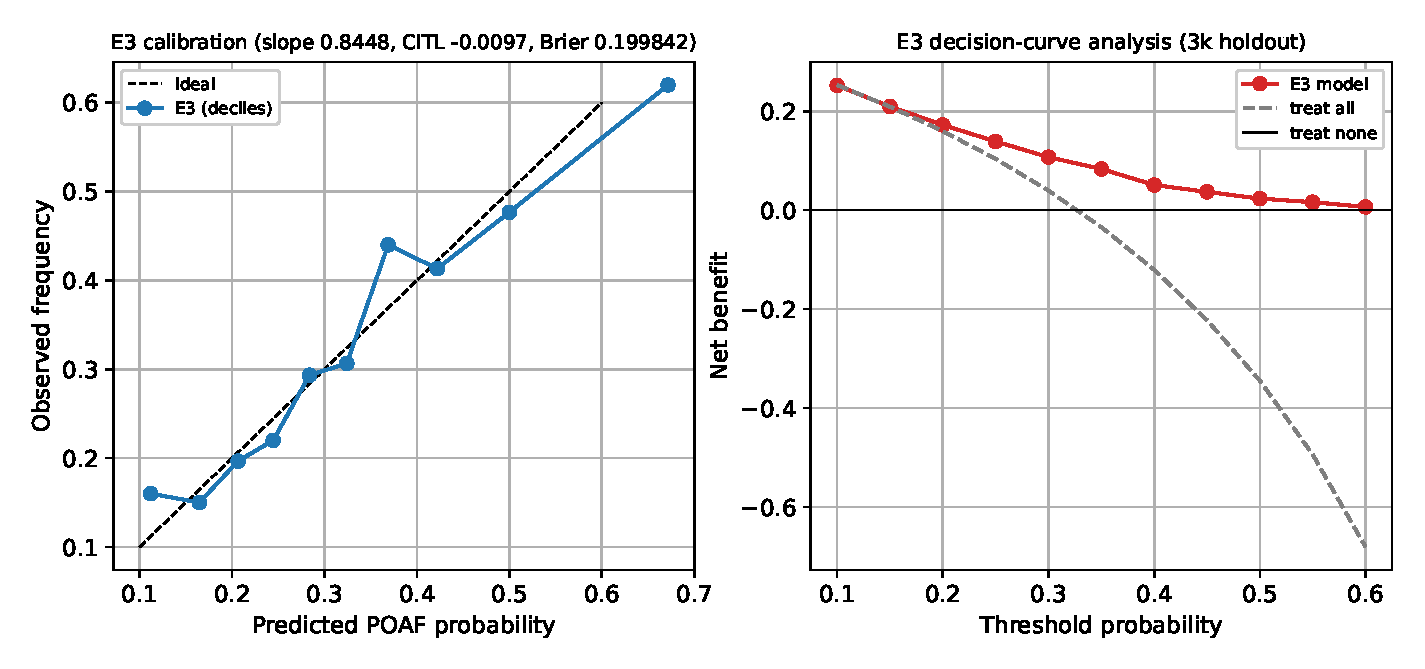
\includegraphics[width=\columnwidth]{figures/fig8_calibration_dca}
\caption{E3 reliability and clinical utility on the 3k holdout. Left: calibration
(reliability) curve across deciles of predicted risk (slope $0.845$, intercept
$-0.113$, calibration-in-the-large $-0.010$, Brier $0.200$). Right: decision-curve
analysis; E3's net benefit (solid) exceeds both treat-all and treat-none across
the clinically relevant threshold range.}
\label{fig:caldca}
\end{figure}

\emph{Explanations.} For clinician trust, predictions must be locally
explainable. SHAP attributions \cite{lundberg2017} and local surrogate
explanations \cite{ribeiro2016} can surface, for an individual patient, the
cohort-specific young-age/inflammation/anemia/valve-burden signals that the
engineered features encode (Section~\ref{sec:features})---turning a
topological-subspace score into a legible narrative, while making explicit that
these signals reflect this cohort's selection structure and may not transport.

\emph{Reporting standards and risk of bias.} Credibility requires conformance to
TRIPOD+AI reporting \cite{collins2024,collins2015} and a PROBAST/PROBAST+AI
risk-of-bias assessment \cite{wolff2019,moons2025}. The EI protocol is
deliberately aligned with these standards: a locked split, folds-internal
preprocessing, a single-use holdout firewall for the final confirmation draw, an
auxiliary-label contract that forbids inference-time leakage, full statistical
inference (95\% CIs and DeLong tests), and a complete receipt corpus together
address the most common sources of optimism and bias that PROBAST flags. We are
explicit that the exploratory evolution series and benchmark ladder used the 3k
holdout repeatedly as a monitor (which is what exposes the winner's curse), so the
single-use guarantee is scoped to the confirmation draw and not claimed for the
whole study. Trust and adoption, ultimately, will follow from this transparency as
much as from the AUROC.

\section{Conclusion}
\label{sec:conclusion}
We set out to test whether the construction of a machine-learning pipeline can be
decomposed, scripted, and searched by an autonomous engineered intelligence---and
whether doing so can move a hard clinical problem. On a fixed STS POAF split, an
EI built from an eight-stage grammar, the ZYAL agent-scripting language, a
supervisor and a fleet of up to 70 agents, genetic evolution with adversarial
judges, and a single-use holdout firewall for the confirmation draw produced a
license-clean champion, E3, at $0.689309$ holdout AUROC (95\% CI
$[0.670, 0.709]$). Under honest inference, E3 \emph{reaches} the registry ceiling
but is statistically indistinguishable from strong human baselines (E3 vs.\ best
human $p{=}0.099$; vs.\ baseline borderline at $p{=}0.048$), and---because it was
itself selected under a noisy CV regime against thousands of competitors---the
winner's curse applies to E3 too. Along the way the system surfaced 24
cohort-specific engineered features (whose dominant young-age theme is a selection
confound, not rediscovered physiology), a well-calibrated and clinically useful
risk model, and a stage attribution that pinpoints fusion as the dominant driver
of the \emph{CV objective}. We are equally clear about the limits: the CV peak at
$0.7317$ is optimism, CV does not rank holdout (Spearman $-0.061$), the
de-duplicated temporal cohort settles every method into $0.680\text{--}0.689$
(with deep trees inflated to $0.78$ only by 24.6\% leaked rows), and $\sim$0.689 is
a genuine wall for registry-only POAF that no amount of search has breached.

The deeper claim is methodological. The headline result is not a better
predictor; it is (i)~an auditable, replayable search that \emph{reaches} the
registry-only POAF ceiling without fooling itself, and (ii)~a clean demonstration
that cross-validation does not rank held-out generalization in this regime, which
is exactly why a firewalled confirmation draw---and not a CV leaderboard---is what
should decide a champion. Literature can be consumed at machine scale, hypotheses
can be generated and validated by the thousand under one leakage-safe contract,
and selection can be made explicit, auditable, and replayable. The honest ceiling
and the CV--holdout decoupling we report are not a defeat of that vision; they are
its first rigorous, reproducible measurement.

\section*{Author Biographies}
\textbf{Jepson Taylor} is affiliated with NeverHuman Search, Scottsdale, AZ, and
works on engineered-intelligence systems for autonomous algorithm discovery,
reproducible evaluation, and clinical-model governance.

\textbf{Zain Khalpey, MD} is a cardiothoracic surgeon at HonorHealth in
Scottsdale, AZ, with clinical and research interests spanning robotic cardiac
surgery, artificial intelligence, regenerative medicine, and advanced heart and
lung surgical care \cite{honorHealthKhalpey}.

\bibliographystyle{IEEEtran}
\bibliography{references}

\end{document}
